% !TEX TS-program = xelatex
% !TEX encoding = UTF-8 Unicode
% !Mode:: "TeX:UTF-8"


% \documentclass[bachelor,nocolorlinks, printoneside]{seuthesis} % 本科
% \documentclass[master]{seuthesis} % 硕士
% \documentclass[doctor]{seuthesis} % 博士

%% 电子版 去除空白页 oneside,openany
\documentclass[engineering,oneside,openany]{seuthesis} % 工程硕士
%%% 打印版
%\documentclass[engineering,printtwoside]{seuthesis} % 工程硕士
\usepackage{CJK,CJKnumb}
\usepackage{amsmath}
\usepackage{amsfonts} 
\usepackage{bm} 
\usepackage{algorithm}
%\usepackage{algorithmic}
\usepackage{algorithmicx}
\usepackage{graphicx}
\usepackage{algpseudocode}
\usepackage{subfigure}
\usepackage{fancybox}
\usepackage{arydshln}
\usepackage{multirow}
\usepackage{url}
\renewcommand{\algorithmicrequire}{ \textbf{Input:}} %Use Input in the format of Algorithm
\renewcommand{\algorithmicensure}{ \textbf{Output:}} %UseOutput in the format of Algorithm

\DeclareCaptionFont{capFont}{\song\wuhao} % 表格名及图名用5号宋体
\DeclareCaptionLabelSeparator{twospace}{~~}
\captionsetup{
	labelsep=twospace,% 去掉图标签后的冒号
	font={capFont},%
	figurename={图},%
	tablename={表},%
	listfigurename={插图目录},%
	listtablename={表格目录}
}
% latex 画图
\usepackage{palatino}
\usepackage{tikz}
\usetikzlibrary{shapes.geometric, arrows}

\newcommand{\tablefontsize}{\fontsize{10pt}{10pt}\selectfont}
\usepackage{array}
\newcommand{\PreserveBackslash}[1]{\let\temp=\\#1\let\\=\temp}
\newcolumntype{C}[1]{>{\PreserveBackslash\centering}p{#1}}
\newcolumntype{R}[1]{>{\PreserveBackslash\raggedleft}p{#1}}
\newcolumntype{L}[1]{>{\PreserveBackslash\raggedright}p{#1}}

%% 自定义
\usepackage{color}
\usepackage{amsthm}

\newtheoremstyle{mystyle}{3pt}{3pt}{\song}{0cm}{\bf\hei}{}{1em}{}  \theoremstyle{mystyle}

\newtheorem{definition}{\hspace{2em}定义}[chapter]
\newtheorem{throrem}{\hspace{2em}定理}[chapter]
\newtheorem{lemma}{\hspace{2em}引理}[chapter]
\newtheorem{example}{\hspace{2em}例子}[chapter]

\usepackage{verbatim}    % 使用注释

\usepackage{booktabs}

\floatname{algorithm}{算法}
\renewcommand{\algorithmicrequire}{\textbf{输入:}}
\renewcommand{\algorithmicensure}{\textbf{输出:}}

% 参考文献引用
\usepackage[numbers,sort&compress]{natbib}
\newcommand{\upcite}[1]{\textsuperscript{\textsuperscript{\cite{#1}}}}
%\usepackage{cite}

% 去掉空白页的页眉和页脚
\usepackage{emptypage}
\cleardoublepage

% 算法编号加上章数
\numberwithin{algorithm}{chapter}


\begin{document}
	\categorynumber{TP339} % 分类采用《中国图书资料分类法》
	\UDC{004.9}            %《国际十进分类法UDC》的类号
	\secretlevel{公开}    %学位论文密级分为"公开"、"内部"、"秘密"和"机密"四种
	\studentid{181698}   %学号要完整,前面的零不能省略。
	
	\title{论文题目}{}{Title of the Thesis}{}
	\author{作者姓名}{Name}
	\advisor{导师姓名}{教授}{Name}{Prof.}
	% 仅专硕有校外导师
%	\coadvisor{校外导师姓名}{高工}{Name}{Senior Engineer} 
	\committeechair{~~~~~~~~~~}%{Jun Feng}{Prof.}
	% 学硕:工学硕士		专硕:工程硕士
	\degree{工学硕士} 
	\major[12em]{专业}
	
	\defenddate{}
%	\authorizedate{2021年\quad 月\quad  日}
	\authorizedate{}
	\department{计算机科学与工程}{School of Computer Science and Engineering}
	\duration{2021年1月—2021年6月}
	\address{}
	\thanks{}
	\maketitle
	
	
	\begin{abstract}{关键词1;关键词2}	

	摘要概括全文,应该包含且仅包含核心问题、工作、方法、算法、结论以及分析结果。

	\end{abstract}
	
	\begin{englishabstract}{Key word 1, key word 2}
		something
		
	\end{englishabstract}
	
	\tableofcontents
	\listoffigures
	\listoftables
	%\listofalgorithms
	

	\begin{terminology}
		
		\begin{table}[h]\centering
%			\caption{深度强化学习术语表}
			\renewcommand\arraystretch{1.5}
			%\Large
			\begin{tabular}
				{L{2.2cm} L{5cm} L{2.2cm} L{5cm}}
%				{>{\normalsize}m{0.2\textwidth} <{\centering}m{0.4\textwidth} <{\centering}m{0.3\textwidth}}
				\hline
				缩略词   &   \multicolumn{2}{l}{英文全称} &   中文全称   \\\hline
				DRL &	\multicolumn{2}{l}{Deep Reinforcement Learning}	& 深度强化学习\\\hline
				\hline
				符号   	&   含义 &符号   	&   含义 \\\hline
				$t$ 	&	时间步$t$& $s_t$		&	时间步$t$的状态 \\\hline
			\end{tabular}
			%\caption{my table}
		\end{table}
		
		
		%\printnomenclature
	\end{terminology}
	
	\begin{Main} % 开始正文
		
		\chapter{可能用得上的模板}
\label{introduction}

\section{引用}

深度强化学习\cite{Mnih2013PlayingAW,Ye2020MasteringCC}中,深度学习用于复杂环境的状态表征,有效抽取图像、仿真等高维连续状态空间的特征;强化学习通过与环境交互获得经验存入经验池,采样经验更新网络,学习最大化期望回报的目标策略\upcite{Silver2016MasteringTG,Li2017DeepRL}。

引用文章使用 cite,引用文章内容使用 upcite,多个引用使用英文逗号间隔。

\section{图片}

\subsection{单张图片}

\begin{figure*}
	\centering
	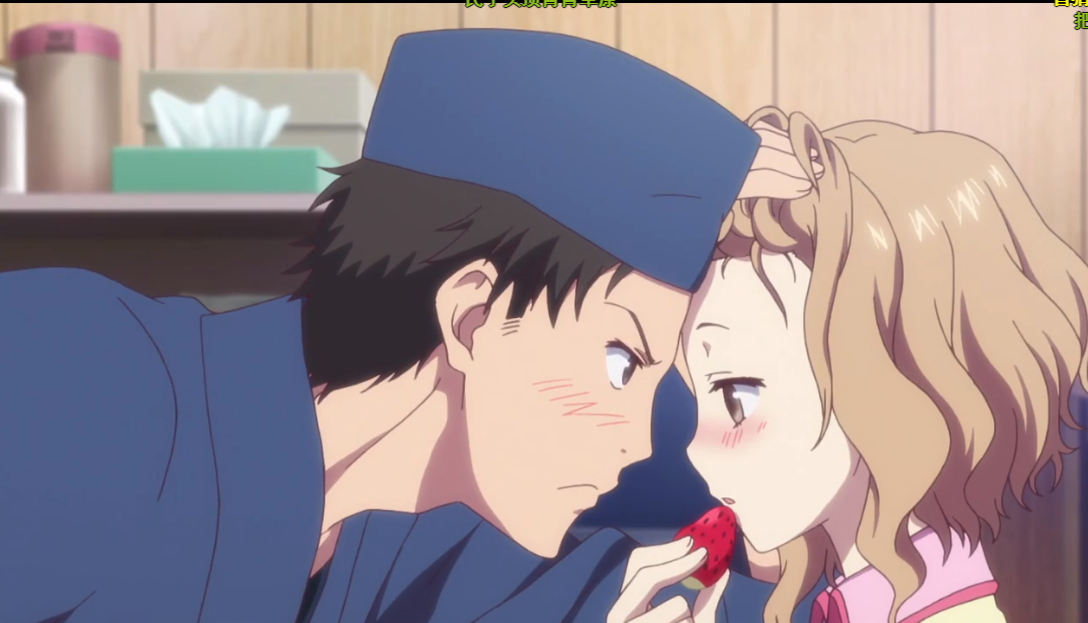
\includegraphics[width=0.7\textwidth]{img/ohana.png}
	\caption{\label{fig:one_fig}单张图片}
\end{figure*}

单张图片如图\ref{fig:one_fig}所示。

\subsection{多张图片}

\begin{figure*}[htbp]
	\centering
	
	\subfigure{
		\begin{minipage}[t]{0.5\linewidth}
			\centering
			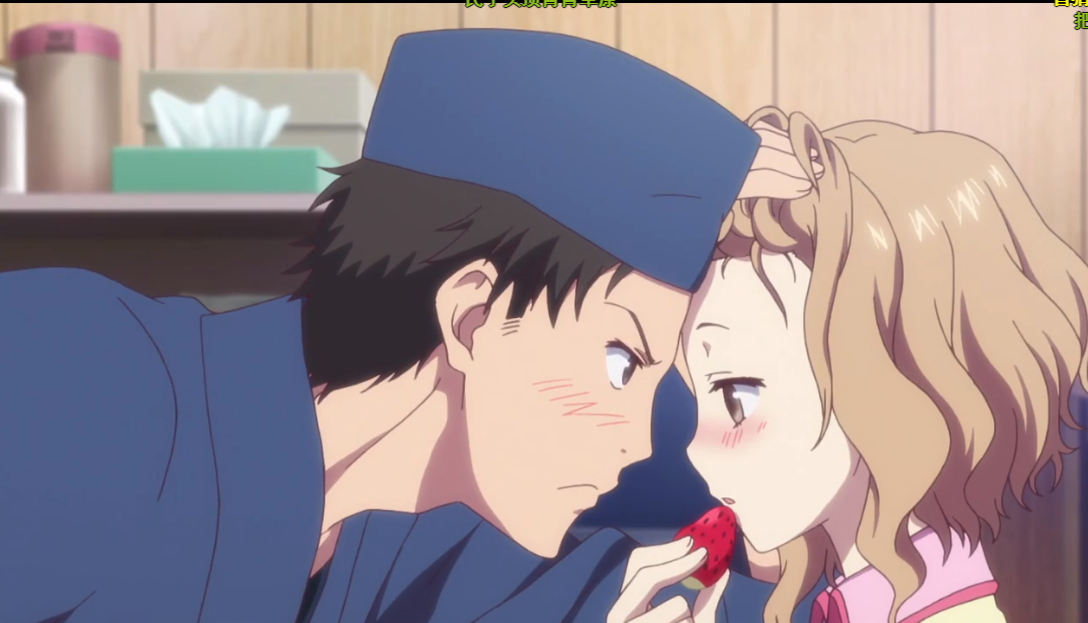
\includegraphics[width=2.8in]{img/ohana.png}\\
			\vspace{0.02cm}
			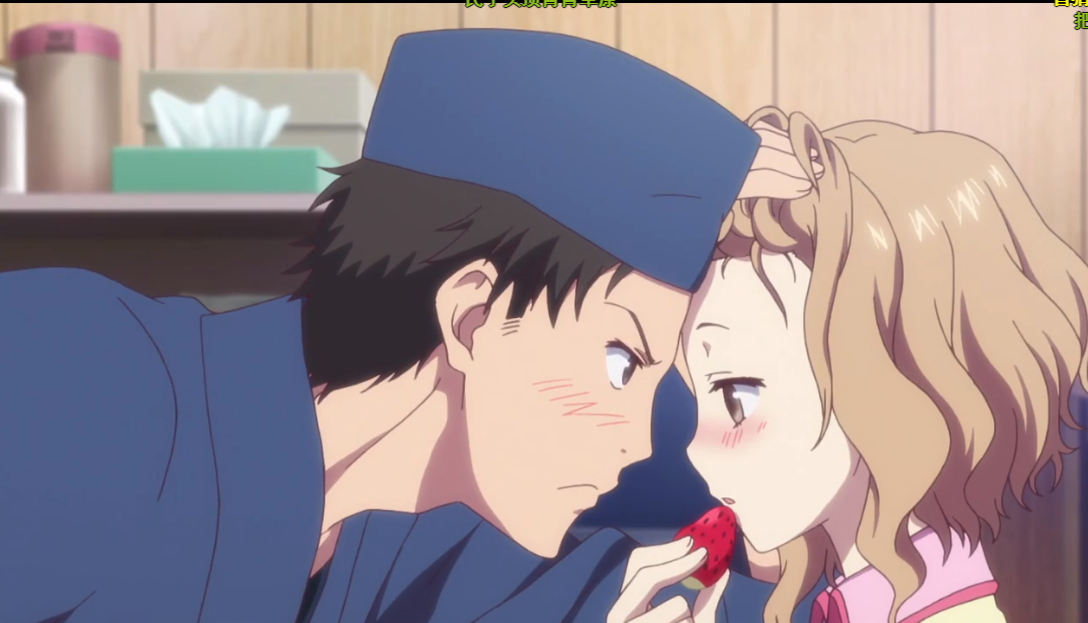
\includegraphics[width=2.8in]{img/ohana.png}\\
			\vspace{0.02cm}
		\end{minipage}%
	}%
	\subfigure{
		\begin{minipage}[t]{0.5\linewidth}
			\centering
			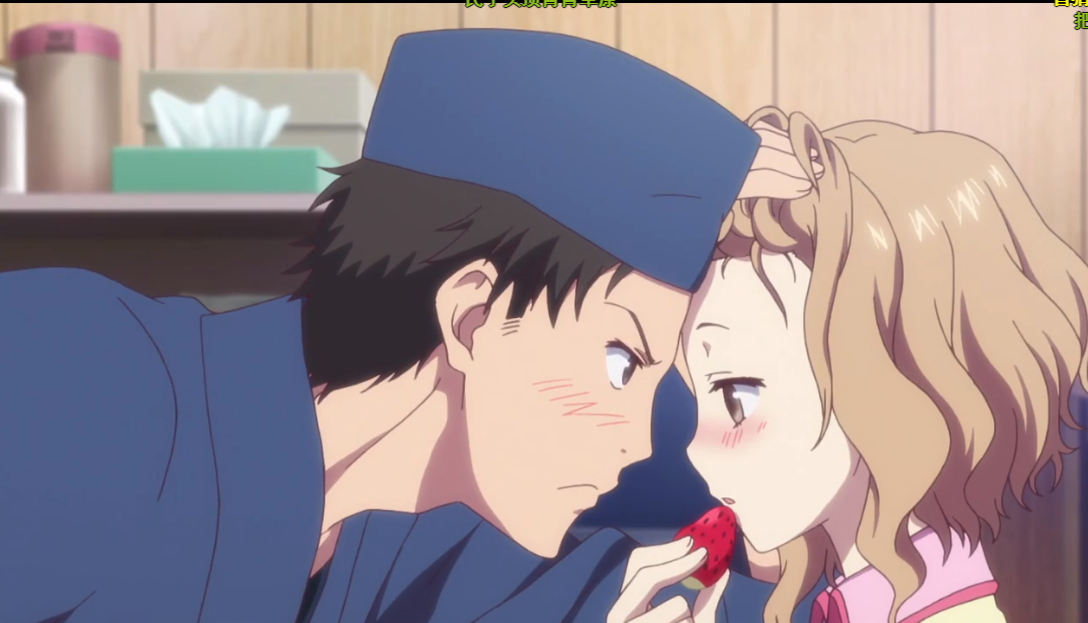
\includegraphics[width=2.8in]{img/ohana.png}\\
			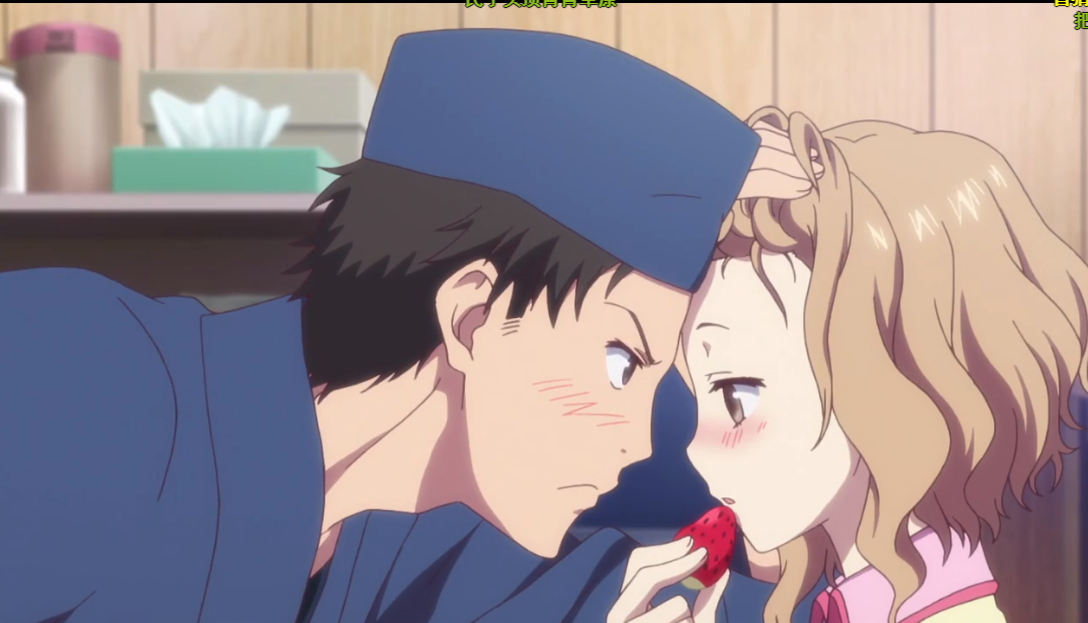
\includegraphics[width=2.8in]{img/ohana.png}\\
		\end{minipage}%
	}%
	
	\centering
	\caption{多张图片}
	\label{fig:multi_fig}
	
\end{figure*}

\newpage
\section{表格}

\subsection{表格一}
表格一如表\ref{tab:tab_1}所示,表格中可以引用参考文献方便阅读。
\begin{table}[htbp]
	\caption{表格一}
	\label{tab:tab_1}
	\renewcommand\arraystretch{1.2}
	%\Large
	\begin{tabular}{L{2.5cm} L{3.2cm} L{4cm} L{4.5cm}}
		%		{>{\normalsize}m{0.2\textwidth} <{\centering}m{0.2\textwidth}<{\centering}m{0.2\textwidth} <{\centering}m{0.3\textwidth}}
		\hline
		方法 	& 经验组成		& 经验池		& 保留优先级			\\
		\hline
		方法一\cite{Mnih2013PlayingAW} & 转移	& 先进先出	 & 时间顺序		\\	
		方法二\cite{Karimpanal2018ExperienceRU} 	& 转移序列	& 先进先出	 & 时间顺序		\\	
		\hline
	\end{tabular}
\end{table}

\subsection{表格二}
表格二如表\ref{tab:tab_2}所示。
\begin{table*}[htbp]
	\centering
	\caption{\label{tab:tab_2}表格二}
	\begin{tabular}
		{C{3cm} C{1.2cm} C{1.5cm}  C{1.2cm} C{1.5cm}  C{1.2cm} C{1.5cm}}
		\hline
		\multirow{2}{*}{数据集}   &   \multicolumn{2}{c}{方法一} &   \multicolumn{2}{c}{方法二} &   \multicolumn{2}{c}{方法三}  \\
		%		\cline{2-9}
		&	指标1 & 指标2 &	指标1 & 指标2&	指标1 & 指标2	\\
		\hline
		数据集1	&	0.975	&	0.53	&	0.983	&	0.56	&	$\bm{1.000}$	&	$\bm{0.32}$	\\
		数据集2	&	0.975	&	0.53	&	0.983	&	0.56	&	$\bm{1.000}$	&	$\bm{0.32}$	\\
		\hline\hline
		平均值	& 0.989	& 0.31	& 0.988	& 0.29	& $\bm{1.000}$	& $\bm{0.17}$ \\
		\hline
	\end{tabular}
\end{table*}

\section{公式}

需要等号对齐的公式写法。

\begin{equation}
\begin{split}
\nabla_{\theta}J(\pi_{\theta})
& = \int_{\mathcal{S}}\rho^{\pi}(s)\int_{\mathcal{A}} \nabla_{\theta}\pi_{\theta}(a|s)Q^{\pi}(s,a)dads \\
& = \mathbb{E}_{s\sim\rho^{\pi},a\sim\pi_{\theta}}[\nabla
_{\theta}\log\pi_{\theta}(a|s)Q^{\pi}(s,a)]
\end{split}
\end{equation}

\section{算法}

算法如算法\ref{algorithm:alg_1}所示。

\begin{algorithm}[htbp]
	\caption{算法}
	\label{algorithm:alg_1}
	\begin{algorithmic}[1]
		\Require 输入数据
		\Ensure 输出结果
		\State 步骤
		\For {时间步t = $0, \dots, T$}
		\State 循环
		\If {判断条件}
		\State 步骤
		\EndIf
		\State 步骤
		\EndFor
	\end{algorithmic}
\end{algorithm}

		
		
	\end{Main} % 结束正文

	
	% 参考文献格式
%	\bibliographystyle{plain}
	\bibliographystyle{ieee}
	% 参考文献文件 后缀为.bib
	\bibliography{ref_1, ref_2}
	
	\newpage
	\printindex % 索引
		
	\begin{Acknowledgement}{}
		致谢
		
		\begin{flushright}
			姓名
			
			2021年5月于南京
		\end{flushright}
	\end{Acknowledgement}
	
	\begin{Resume}
		个人介绍
		
		\subsection*{硕士期间发表的学术论文}
%		\begin{enumerate}
			
			[1] 论文名称 [J]. 东南大学计算机科学与工程学院 2021 年研究生学术论坛,2021.
			
%		\end{enumerate}
		
		\subsection*{硕士期间参与的研究项目}
		\begin{enumerate}
			\item xxxxx		
		\end{enumerate}
	\end{Resume}
	
	
	
\end{document}
